\documentclass[12pt]{article}
\usepackage[breaklinks=true]{hyperref}
\usepackage[margin=0.5in]{geometry}
 
\usepackage{graphicx} %package to manage images
%\graphicspath{ {./images/} }

\usepackage{color}

\definecolor{pblue}{rgb}{0.13,0.13,1}
\definecolor{pgreen}{rgb}{0,0.5,0}
\definecolor{pred}{rgb}{0.9,0,0}
\definecolor{pgrey}{rgb}{0.46,0.45,0.48}

\usepackage{listings}
\lstset{language=Java,
  showspaces=false,
  showtabs=false,
  tabsize=2,
  breaklines=true,
  showstringspaces=false,
  breakatwhitespace=true,
  commentstyle=\color{pgreen},
  keywordstyle=\color{pblue},
  stringstyle=\color{pred},
  basicstyle=\ttfamily\small,
  frame=single,
  moredelim=[il][\textcolor{pgrey}]{$$},
  moredelim=[is][\textcolor{pgrey}]{\%\%}{\%\%}
}

\title{\textbf{Exam Prep:} PPM Image Manipulation in Java}
\author{
	Melvyn Ian Drag
}
\date{\today}


\begin{document}
\maketitle

\begin{abstract}
In this class we will play around with the ppm image format so you have more confidence and ability to be able to complete the midterm exam.
\end{abstract}


\section{It's Hard to Find a Good Greenman}
Last week we used a \textit{greenman.png} image to do some image manipulation tasks. This week we will focus on \textit{.ppm} images - but where do we find a good one to play with? Use \textbf{imagemagick}. Note that imagemagick is a command line tool that is popular among linux and macOS users - I don't know if windows users like it or not, though I think you can download it. Anyway, I want to change the 
mage from \textit{png} format to \textit{ppm}. Here's what the command looks like. If you're on Linux or Mac, you might want to check this program out because it is very userful. Here's how I convert to ppm:

\begin{lstlisting}
melvyn@thinkpad$ convert greenman.png greenman_bin.ppm
melvyn@thinkpad$ head -n4 greenman_bin.ppm
# a bunch of unreadable junk
# this is because the image is in BINARY ppm format. Check the ppm
# specification here and see that P6 is a binary format
# https://en.wikipedia.org/wiki/Netpbm_format
melvyn@thinkpad$ head -n1 greenman_bin.ppm
P6
\end{lstlisting}

For our purposes, we want to use the image in ASCII format, not binary. So I do the command like this:

\begin{lstlisting}[language=bash]
$ convert greenman.png -compress none greenman_ascii.ppm
$ head -n4 greenman_ascii.ppm
P3
WxH
255
... a bunch of numbers between 0 - 255 written in ASCII.
\end{lstlisting}

And that, boys and girls is the story of how I got this great greenman we are using today. I documented the steps just to show you how these types of problems are solved. Now we move on to viewing the image.

\section{Let's see some ppm files}
I want you to see the ppm with your own eyes so you know that it is indeed an image. During lecture I will use our friend \textit{eog} to view it. \textit{imagemagick} also supports ppm files. I don't know about your favorite Windows tools. You can try. 

\begin{center}
\textbf{Have students try to view the greenman.ppm file - if they cannot allow them to come up and use my laptop. Can anyone find a good Windows ppm file viewer?}
\end{center}

Here are the two ppm files that we will focus on in today's lecture.

\begin{figure}[h]
  \centering
    
\includegraphics[width=0.1\textwidth]{greenman.png}
  \caption{greenman.ppm before transformation}
\end{figure}

\begin{figure}[h]
  \centering
    
\includegraphics[width=0.1\textwidth]{output.png}
  \caption{greenman.ppm after transformation}
\end{figure}


\section{Exercise \#1a}
The first exercise we will do in class today is have you comment a bit of java code. 

The code of interest is the \textit{Code/Exercise1/ChangeBackground.java} file from the class repository. The code must be compiled and run along with the \textit{Code/Exercise2/ClassAssignment.java} file, which is the main file that runs the background-changing functions.

This code reads a \textit{.ppm} image and turns all the white background pixels into red pixels.

\subsection{ Comment Styling Requirements }
I spoke to a bunch of people in class and they told me that the midterm was quite hard - so I wrote ppm handling code myself and I just want you to read it and document what it does and how it does it. They say you can learn alot about software by reading other people's code. For this exercise you must comment the code I wrote such that every function has a comment in the form:

\begin{verbatim}
/**
 * Brief description of what function does
 *
 * @param paramName1 - description of parameter
 * @param paramName2 - description of parameter
 * @param etc.
 * @throws exceptiontype - circumstance under which it is thrown
 * @throws exceptiontype2  - circumstance under which it is thrown
 * @return description of the return value e.g. is it a string, 
 *         is a HashMap, what does it represent, etc.
 *
 * And here goes a more detailed description of the function and
 * how it works. If the function happens to use a special algorithm,
 * describe it. If the function relies on the ARGB channel values of 
 * an image being stored in a single 4 byte int, say that. The idea of 
 * this section is that someone who reads the code can understand it 
 * better.
 */
\end{verbatim}

\subsection{Example}
Here is an example:

\lstinputlisting{PrintString.java}

\section{Exercise \#1b}

Take the code provided in class, and have it turn the greenman.ppm file into a blueman.ppm file. Change all the green pixels to blue.

\section{Grading for Exercise 1}
When you have successfully completed exercises \#1a and \#1b, submit your zipped Java files on blackboard. Show me your code working on your computer and I'll grade you on blackboard. I just need the submission so I have a reference of your work if there is any dispute about your grade later.

\section{Exercise \#2}

Make all of the functions in \textit{Code/Exercise2/BitShift.java} return `true'. Note when I compile all the files ( BitShift.java, LeftShifter.java, RightShifter.java, OtherLeftShifter.java and Shifter.java ) and run, the code prints out 'false'. Make it print `true' ( without changing the value of `myInt' in the code!! You need to pass the appropriate ExpectedValue to each function call. You'll need a pencil and paper to figure this out ( there are other ways, but the most effective way for you to master bit shifting is using a pencil and paper to figure things out ).

\begin{figure}[h]
  \centering
    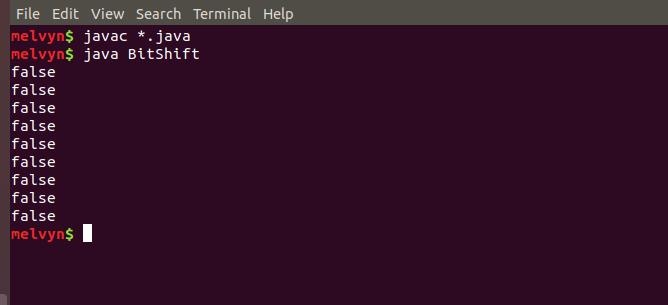
\includegraphics[width=0.5\textwidth]{Exercise2.png}
  \caption{Code doesn't say `true' yet :(}
\end{figure}

\subsection{HINT!!!}

The binary for 

\begin{center}
0xFF6F8F90
\end{center}

is

\begin{center}
11111111011011111000111110010000
\end{center}

\section{Grading for Exercise 2}

Show me your code working. Show me the work you did with paper and pencil. Submit on blackboard. I'll grade it in class.

\section{Coming Up In Class}

We've had some technical difficulties in this class, so we're running a bit behind schedule. That's fine so long as you're learning. So far I feel like people understand inheritance and primitive types more or less. This lecture will put an end to our discussion of bitwise operators and image processing. I have a bunch of dreams for the class, we'll get to as much of the following as possible:

\begin{enumerate}
\item Look at Collections like \textit{HashMap}, \textit{ArrayList}, \textit{etc.}
\item Take a deeper look at the magic behind the Java string class
\item Look more at Pass by Value vs Pass by Reference and how Java classes work in memory
\item Learn about concurrent programming, making your code do many things simultaneously
\item Make some music with Java
\item Do some basic graphics programming 
\item Do some basic statistical analysis with Java of a few VERY interesting datasets
\item Make a little website with Java
\end{enumerate}

I'm having fun in class so far, hope you feel like you are learning alot about programming from this class. We'll do as much as we can in our few remaining weeks.

\end{document}
